\documentclass[border=3pt]{standalone}
\usepackage{amsmath,amssymb,mathptmx,graphicx,tikz}
\usetikzlibrary{arrows.meta,calc}
\begin{document}
\begin{tikzpicture}[>=Stealth,font=\fontsize{8.5}{10.5}\selectfont,
 panel/.style={draw=black,line width=.6pt,minimum width=3.65cm,minimum height=3.05cm},
 flow/.style={->,line width=.8pt}]
\foreach \x/\heading in {0/Timed reference,4.25/Geometric feedback,8.5/Rotor allocation,12.75/Quadrotor dynamics}{
 \node[panel] at (\x,0) {};
 \node[font=\bfseries\fontsize{10}{12}\selectfont] at (\x,1.20) {\heading};
}
\begin{scope}[shift={(0,.05)}]
 \draw[gray,dashed] (0,0) ellipse[x radius=.83,y radius=.56];
 \draw[->,gray] (-1.15,-.65)--(1.1,-.65) node[right,black] {$x$};
 \draw[->,gray] (-1.15,-.65)--(-1.15,.65) node[above,black] {$y$};
 \fill (.59,.40) circle (1.7pt);
 \draw[flow] (.59,.40)--(1.10,-.05);
 \node[above] at (.91,.43) {$v_d$};
 \draw[->] (0,0)--(.59,.40) node[midway,above left] {$r$};
 \node at (0,-1.05) {$x_d,\;v_d,\;a_d,\;\psi_d$};
\end{scope}
\node[align=center] at (4.25,.43) {$e_x=x-x_d,\quad e_v=v-v_d$\\[4pt]
 Position and attitude errors};
\node[align=center] at (4.25,-.62) {$b_{3d}=A/\|A\|$\\[4pt]
 $f=A^\mathrm{T}Re_3,\quad M\in\mathbb{R}^3$};
\node[align=center] at (8.5,.35) {$u=F_a^{-1}\begin{bmatrix}f\\M\end{bmatrix}$};
\node[align=center] at (8.5,-.72) {$\omega_i=\operatorname{sgn}(u_i)\sqrt{|u_i|}$\\[5pt]Four signed rotor commands};
\node at (12.75,.10) {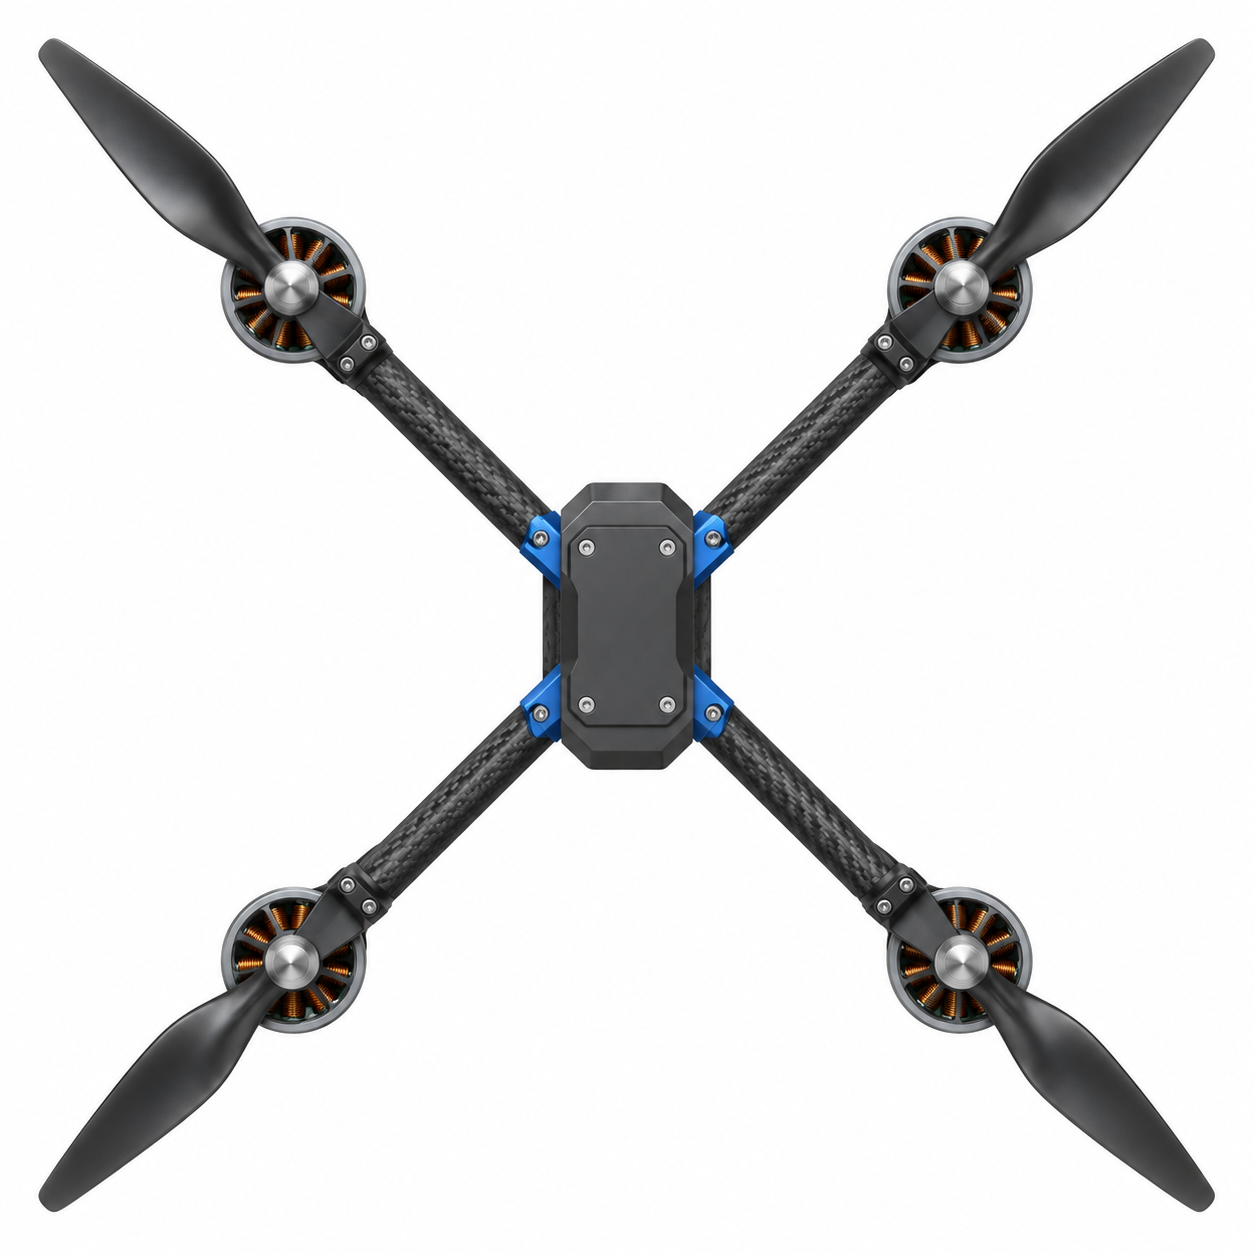
\includegraphics[width=1.85cm]{figures/quadcopter_top.png}};
\node at (12.75,-1.06) {$x,\;v,\;R,\;\Omega$};
\foreach \x in {1.825,6.075,10.325}{\draw[flow] (\x,0)--++(.60,0);}
\draw[flow,dashed] (12.75,-1.525)--(12.75,-2.02)--(4.25,-2.02)--(4.25,-1.525);
\node[fill=white,inner sep=3pt] at (8.5,-2.02) {State feedback: position, velocity, attitude and body rate};
\end{tikzpicture}
\end{document}
